\documentclass[tikz]{standalone}
\usepackage{pgfplots}
\pgfplotsset{compat=1.15}
\usepackage{mathrsfs}
\usetikzlibrary{arrows,calc}
\usepackage{tkz-euclide}

\pagestyle{empty}

\definecolor{AngleClr}{rgb}{0,0.39215686274509803,0}
\definecolor{ShapeClr}{rgb}{0.6,0.2,0}
\definecolor{SecondAngleClr}{RGB}{166, 7, 7}


\begin{document}

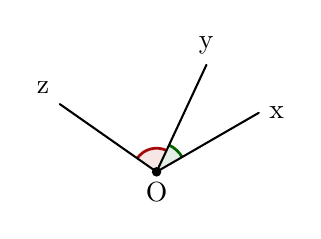
\begin{tikzpicture}[scale=.75]
\tkzSetUpLine[line width=1pt,color=black]
\tkzSetUpPoint[fill=black]

\tkzDefPoints{0/0/B}

\tkzDefPoint(65:2){A}
\tkzDefPoint(30:2){C}
\tkzDefPoint(145:2){D}


\tkzFillAngle[fill=AngleClr,size=.5,fill opacity=0.1](C,B,A)
\tkzMarkAngle[line width=1pt,size=.5,color=AngleClr](C,B,A)

\tkzFillAngle[fill=SecondAngleClr,size=.4,fill opacity=0.1](A,B,D)
\tkzMarkAngle[line width=1pt,size=.4,color=SecondAngleClr](A,B,D)


\tkzDrawPoints[size=3](B)
\tkzLabelPoint[above](A){$\rm y$}
\tkzLabelPoint[below](B){$\rm O$}
\tkzLabelPoint[right](C){$\rm x$}
\tkzLabelPoint[above left](D){$\rm z$}

\tkzDrawSegment[line width=0.75pt](A,B)
\tkzDrawSegment[line width=0.75pt](B,C)
\tkzDrawSegment[line width=0.75pt](B,D)

\end{tikzpicture}

\end{document}
